\section{Технологический раздел} \label{tech}

В данном разделе выбраны и обоснованы средства реализации, работана база данных, а также будет разработан интерфецс доступа к данным. Выполнено покрытие тестами публичного API приложение, протестирован триггер.


\subsection{Выбор объектной базы данных}

При выборе объектной базы данных стоит помнить, что использоваться она будет для хранения приложений (бинарных файлов) объемом до 10МБ. Ниже представлен обзор существующих решений и обоснование выбора базы данных.

\subsubsection{Microsoft Azure Blob Storage}

Microsoft Azure Blob Storage - это облачное хранилище данных, предоставляемое компанией Microsoft в рамках облачного сервиса Azure. Azure Blob Storage предназначено для хранения больших объемов неструктурированных данных, таких как файлы, изображения, видео, аудио, резервные копии, журналы и другие типы информации. Это расширяемое и высокодоступное хранилище, которое обеспечивает надежное хранение данных в облаке с возможностью масштабирования по требованию.

Основной недостаток -- недоступна для использования в России.


\subsubsection{Yandex S3}

Amazon Simple Storage Service (Amazon S3) --- это облачное хранилище данных, предоставляемое Amazon Web Services (AWS). S3 предоставляет возможность хранить и извлекать любое количество данных в Интернете, обеспечивая высокую доступность, надежность и масштабируемость.

Основные характеристики Amazon S3:

\begin{enumerate}
	
	\item доступность и надежность: S3 обеспечивает высокую доступность данных и надежность, гарантируя, что ваши данные будут доступны в любое время;
	
	\item масштабируемость: S3 позволяет хранить огромные объемы данных без необходимости заботиться о масштабировании инфраструктуры;
	
	\item управление данными: Вы можете управлять доступом к вашим данным, устанавливать права доступа, шифровать данные и использовать другие функции для обеспечения безопасности информации;
	
	\item стоимость: Вы платите только за использование, что делает S3 экономически выгодным решением для хранения данных.
\end{enumerate}

Amazon S3 широко используется для хранения резервных копий, статических сайтов, медиафайлов, архивов данных, а также для обработки и анализа больших объемов информации.

Yandex S3 предоставляет совместимый с <<оригинальным>> Amazon S3 программный интерфейс и доступен в России. В современной мирк s3 является де-факто стандартом хранения бинарных файлов.

\subsubsection{Резальтат выбора объектной базы данных}

Для реализации проекта среди 2 рассмотренных вариантов была выбрана база данных Yandex S3, так как она доступна в России и удовлетворяет всем требованиям.


\subsection{Выбор реляционной базы данных}

Ниже представлен обзор существующих решений обоснование выбора базы данных.

\subsubsection{Oracle Database}

Oracle Database - это одна из самых популярных и мощных реляционных баз данных, разработанная компанией Oracle Corporation. Она широко используется в корпоративных средах для хранения и управления данными, обеспечивая высокую производительность, надежность и масштабируемость. Основным недостатком, который делает невохможным применения данной базы данных является отсутствие поддержки этой базы данных выбранным для разработки фреймворком userver.


\subsubsection{MySQL}

MySQL - это одна из самых популярных открытых реляционных баз данных, широко используемая веб-разработчиками и предприятиями для хранения и управления данными. Тем не менее, в рамках данном работы получилось выделить следующие минусы данной системы управления базами данных: 

\begin{enumerate}
	\item ограниченная поддержка даты и времени: MySQL имеет ограниченный набор типов данных для работы с датой и временем, что может вызывать сложности при работе с различными форматами даты и времени или при работе с часовыми поясами;
	\item ограниченные возможности хранения текстовых данных: MySQL имеет ограничения на размер текстовых полей, что может быть проблемой при работе с большими объемами текстовых данных, таких как скрипты выступлений, отправленные через комментарии.
\end{enumerate}

Хотя MySQL является мощной и гибкой базой данных, ограниченный набор типов данных может стать препятствием к применению в данном проекте.


\subsubsection{PostgreSQL}

PostgreSQL - это мощная и расширяемая объектно-реляционная система управления базами данных (СУБД), которая широко используется в различных проектах и приложениях. Она является открытой и бесплатной для использования, что делает ее популярным выбором среди разработчиков и организаций. 

PostgreSQL предлагает широкий набор встроенных и сторонних расширений, которые позволяют расширять функциональность базы данных с помощью пользовательских функций, типов данных, операторов и других возможностей. PostgreSQL обеспечивает высокий уровень транзакционной безопасности благодаря поддержке ACID-свойств (атомарность, согласованность, изолированность, долговечность) и механизмам контроля целостности данных.

Из минусов PostgreSQL обычно выделяют отсутствие встроенной возможности шардирования, а также сложность настройки кластера базы данных. В рамках данной работы шардирование не планируется к использованию, а PostgreSQL будет развернута на единичной инсталляции, а не в кластере.

\subsubsection{Результат выбора реляционной базы данных}

В качестве основной базы данных принято использовать PostgreSQL, так как она удовлетворяет заданным требованиям и, кроме того, выбранный для разработки фреймворк userver имеет лучшую поддержку именно этой базы данных.

\subsection{Сущноти объектной базы данных}

Единственная сущность объектной базы данных --- бинарный файл. Доступ к нему осуществляется по имени файла. Имя файла --- его идентификатор (полу в таблице file{\_}meta).

Проектирование ролейвой модели для объектной базы данных разрабатываемого приложения нецелесообрвзно.

\subsection{Сущноти основной базы данных}

Ниже представлены разработанные сущности базы данных.

\subsubsection{Таблицы}

На рисунке \ref{fig:dr-er} представлены сущности-таблицы полученной базы данных. Для обеспечения целостности данных используются внешние ключи, ограничения на уникальность первичного ключа.

\begin{figure}[h!]
	\centering{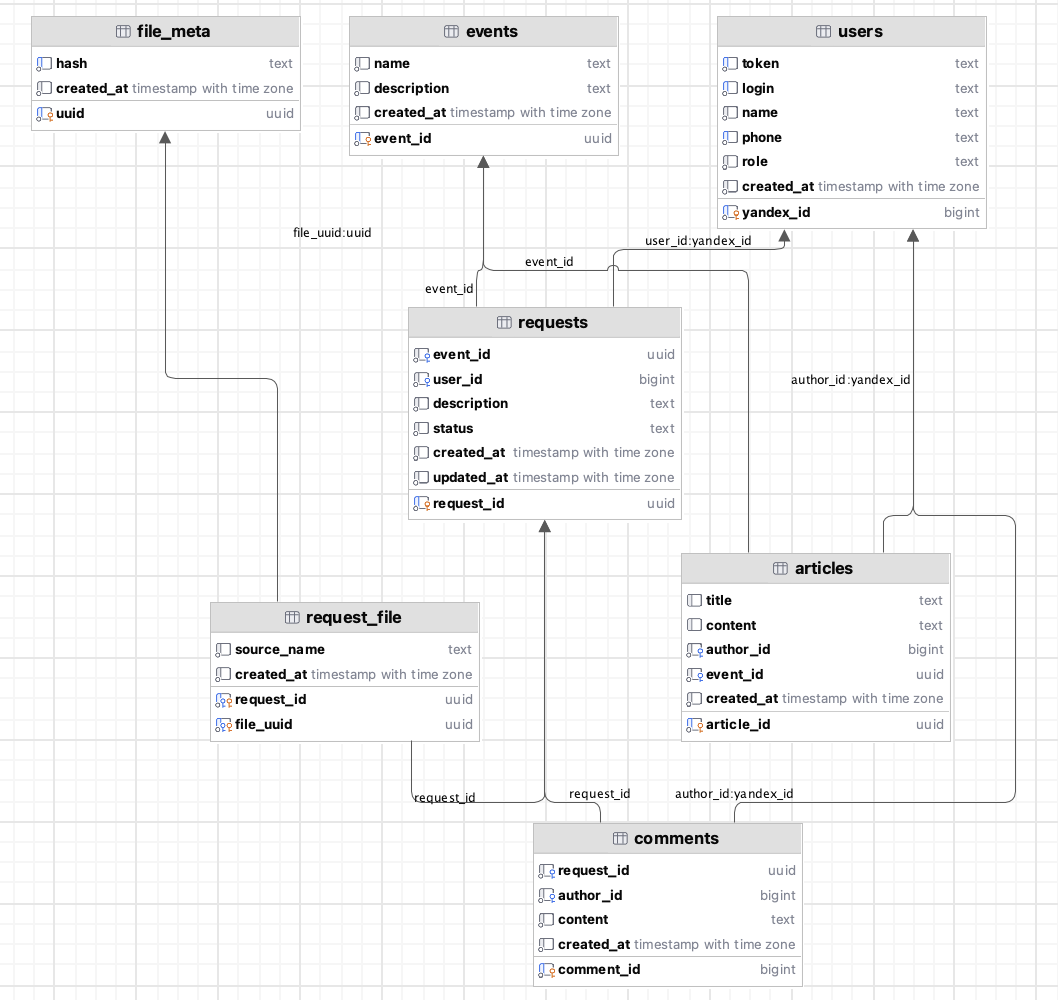
\includegraphics[scale=0.5]{img/db-er.png}}
	\caption{ER-диаграмма базы данных}
	\label{fig:dr-er}
\end{figure}

\subsubsection{Индекс}

В таблице requests используется стандартный b-tree индекс на поле user{\_}id. Использование необходимо обеспечения быстродействия запроса из листинга \ref{lst:exec_time} и для проведения исследования.


\subsubsection{Триггер}

Ниже на рисунке представлена диаграмма спроектированного триггера.

Триггер гарантирует корректность метки времени updated{\_}at таблицы requests. Для тестирования триггера написаны функциональные тесты на языке Python c использованием библиотеки pytest. В таблице \ref{tab:trigger_tests} приведены сценарии тестирования.

\begin{table}[ht!]
	\centering
	\caption{\label{tab:trigger_tests} Сценарии тестирования триггера}
	\begin{tabular}{|l|l|l|l|l|}
		\hline
		\textbf{Событие} & \textbf{Ожидаемый результат} & \textbf{Рельный результат}\\
		\hline
		Изменилось поле description & updated{\_}at = now() & updated{\_}at = now() \\
		\hline
		Изменилось поле status & updated{\_}at = now() & updated{\_}at =  now() \\
		\hline
		Попытка изменить updated{\_}at & updated{\_}at = now() & updated{\_}at =now() \\
\hline
		
	\end{tabular}
\end{table}

\subsubsection{Роли}

Помимо ролевой модели на уровне приложения разработана для дополнительных гарантий безопасности дополнительно разраотана ролевая модель на уровне приложения.  Права пользователей представлены в таблице \ref{tab:roles}.

\begin{table}[ht!]
	\centering
	\caption{\label{tab:roles} Ролевая модель на уровне базы данных}
	\begin{tabular}{|l|l|l|l|l|}
		\hline
		\textbf{Действие} & \textbf{Таблица} & \textbf{everybody} & \textbf{modarator} &  \textbf{admin}\\
		\hline
		select & все таблицы & да & да & да \\
		\hline
		insert, update & requests & да & да & да \\
		\hline
		insert, update, delete & events & нет & да & да \\
		\hline
		insert, update & users & да & да & да \\
		\hline
		insert, update, & requests{\_}file{\_}meta & да & да & да \\
		\hline
		insert, update & file{\_}meta & да & да & да \\
		\hline
		insert, update, delete & permisisions & нет & нет & да \\
		\hline
		insert, update & comments & да & да & да \\
		\hline

	\end{tabular}
\end{table}

Такая ролевая модель на уровне базы данных обеспечит пользователей минимальными необходимыми правами для доступа к просмотру и модификации данных.

\subsection{Интерфейс доступа к данным}

Доступ к данным осуществлдяется методом отправки http запроса на сервер, на котором развернуто приложение. Ниже приведено опсание эндпоинтов.

\begin{enumerate}
	\item /v1/request GET --- получение информации о запросе по его идентификатору. 
	\item /v1/requests GET --- получение информации о всех запросах, доступных для просмотра.
	\item /v1/requests POST --- создание/обновление запроса.
	\item /v1/request/status PATCH --- обновление статуса заявки.
	\item /v1/request/comment POST --- добавление комментария к заявке.
	\item /v1/file GET --- получение файла по его идентификтору.
	\item /v1/file POST --- добавление файла (приложения).
	\item /v1/events GET --- просмотр списка мероприятий.
	\item /v1/event POST --- создание мероприятия.
	\item /v1/event DELETE --- удаление мероприятия.
\end{enumerate}

\subsection{Вывод}

Разработаны и протестированы сущности базы данных, разработан интерфейс взаимодействия с данными.

\pagebreak